\documentclass[12pt, titlepage]{article}

\usepackage[section]{placeins}
\usepackage{ulem}
\usepackage{fullpage}
\usepackage[round]{natbib}
\usepackage{multirow}
\usepackage{booktabs}
\usepackage{tabularx}
\usepackage{graphicx}
\usepackage{float}
\usepackage{hyperref}

\DeclareRobustCommand{\hsout}[1]{\texorpdfstring{\sout{#1}}{#1}}

\hypersetup{
    colorlinks,
    citecolor=black,
    filecolor=black,
    linkcolor=red,
    urlcolor=blue
}



\newcounter{acnum}
\newcommand{\actheacnum}{AC\theacnum}
\newcommand{\acref}[1]{AC\ref{#1}}

\newcounter{ucnum}
\newcommand{\uctheucnum}{UC\theucnum}
\newcommand{\uref}[1]{UC\ref{#1}}

\newcounter{mnum}
\newcommand{\mthemnum}{M\themnum}
\newcommand{\mref}[1]{M\ref{#1}}

\title{SE 3XA3: Module Guide\\TankWar}

\author{Team \#212, Genius
		\\Di Wu, 400117248, wud43 
		\\Jiahao Zhou, 400082351, zhouj56 
		\\Xinyu Huang, 400120376, huangx65
}

\date{\today}


\begin{document}

\maketitle

\pagenumbering{roman}
\tableofcontents
\listoftables
\listoffigures

\begin{table}[bp]
\caption{\bf Revision History}
\begin{tabularx}{\textwidth}{p{3cm}p{2cm}X}
\toprule {\bf Date} & {\bf Version} & {\bf Notes}\\
\midrule
13 March 2020 & 1.0 & Creates the first version of MG\\
\textcolor{red}{4 April 2020} & \textcolor{red}{2.0} & \textcolor{red}{fixed some errors following the TA's comments, merged positionType module and Map module into one and a new module called MapEditTank is added. The use relation graph is slightly changed due to the module changes.}\\

\bottomrule
\end{tabularx}
\end{table}

\newpage

\pagenumbering{arabic}

\section{Introduction}

This project is to re-implement the open source project of BattleCity. The project is 2-D game allows two player to participate in and the game should work on Windows system(Win 7 and later versions) and Mac OS X systems with python and pygame.\\
Our design follows the rules layed out by \citet{ParnasEtAl1984}, as follows:
\begin{itemize}
\item System details that are likely to change independently should be the
  secrets of separate modules.
\item Each data structure is used in only one module.
\item Any other program that requires information stored in a module's data
  structures must obtain it by calling access programs belonging to that module.
\end{itemize}

After completing the first stage of the design, the Software Requirements
Specification (SRS), the Module Guide (MG) is developed~\citep{ParnasEtAl1984}. The MG
specifies the modular structure of the system and is intended to allow both
designers and maintainers to easily identify the parts of the software.  The
potential readers of this document are as follows:

\begin{itemize}
\item New project members: This document can be a guide for a new project member
  to easily understand the overall structure and quickly find the
  relevant modules they are searching for.
\item Maintainers: The hierarchical structure of the module guide improves the
  maintainers' understanding when they need to make changes to the system. It is
  important for a maintainer to update the relevant sections of the document
  after changes have been made.
\item Designers: Once the module guide has been written, it can be used to
  check for consistency, feasibility and flexibility. Designers can verify the
  system in various ways, such as consistency among modules, feasibility of the
  decomposition, and flexibility of the design.
\end{itemize}

The rest of the document is organized as follows. Section
\ref{SecChange} lists the anticipated and unlikely changes of the software
requirements. Section \ref{SecMH} summarizes the module decomposition that
was constructed according to the likely changes. Section \ref{SecConnection}
specifies the connections between the software requirements and the
modules. Section \ref{SecMD} gives a detailed description of the
modules. Section \ref{SecTM} includes two traceability matrices. One checks
the completeness of the design against the requirements provided in the SRS. The
other shows the relation between anticipated changes and the modules. Section
\ref{SecUse} describes the use relation between modules.

\section{Anticipated and Unlikely Changes} \label{SecChange}

This section lists possible changes to the system. According to the likeliness
of the change, the possible changes are classified into two
categories. Anticipated changes are listed in Section \ref{SecAchange}, and
unlikely changes are listed in Section \ref{SecUchange}.

\subsection{Anticipated Changes} \label{SecAchange}

Anticipated changes are the source of the information that is to be hidden
inside the modules. Ideally, changing one of the anticipated changes will only
require changing the one module that hides the associated decision. The approach
adapted here is called design for
change.

\begin{description}
\item[\refstepcounter{acnum} \actheacnum \label{collide}:] How to determine the collide results between two objects.
\item[\refstepcounter{acnum} \actheacnum \label{StateDoubleLife}:] The states of the double life tank.
\item[\refstepcounter{acnum} \actheacnum \label{StateHighSpeed}:] The states of the high speed tank.
\item[\refstepcounter{acnum} \actheacnum \label{StateFastBullet}:] The states of the fast bullet tank.
\item[\refstepcounter{acnum} \actheacnum \label{GeneralDateTank}:] The general data of a tank.
\item[\refstepcounter{acnum} \actheacnum \label{stepCounter}:] How the time is determined.
\item[\refstepcounter{acnum} \actheacnum \label{tankConMove}:] How to determine whether the tank can continue moving.
\item[\refstepcounter{acnum} \actheacnum \label{loadNsaveMap}:] How to load and save the map as a text file.
\end{description}

\subsection{Unlikely Changes} \label{SecUchange}

The module design should be as general as possible. However, a general system is
more complex. Sometimes this complexity is not necessary. Fixing some design
decisions at the system architecture stage can simplify the software design. If
these \textcolor{red}{\sout{decision should later need to be changed}} \textcolor{red}{decisions need to be changed later}, then many parts of the design
will potentially need to be modified. Hence, it is not intended that these
decisions will be changed.

\begin{description}
\item[\refstepcounter{ucnum} \uctheucnum \label{InputOupt}:] Input/output device. (Keyboard)
\item[\refstepcounter{ucnum} \uctheucnum \label{RulePVP}:] The rules of PVP gaming mode.
\item[\refstepcounter{ucnum} \uctheucnum \label{RulePVE}:] The rules of PVE gaming mode.
\item[\refstepcounter{ucnum} \uctheucnum \label{MapStorage}:] Storage of map, including the file style and the location. 

\end{description}

\section{Module Hierarchy} \label{SecMH}

This section provides an overview of the module design. Modules are summarized
in a hierarchy decomposed by secrets in Table \ref{TblMH}. The modules listed
below, which are leaves in the hierarchy tree, are the modules that will
actually be implemented.

\begin{description}
\item [\refstepcounter{mnum} \mthemnum \label{M1}:] Hardware Hiding Modules
\item [\refstepcounter{mnum} \mthemnum \label{M2}:] myTankControl Module
\item [\refstepcounter{mnum} \mthemnum \label{M3}:] Screen Module
\item [\refstepcounter{mnum} \mthemnum \label{M4}:] display Module
\item [\refstepcounter{mnum} \mthemnum \label{M5}:] PvsE Module
\item [\refstepcounter{mnum} \mthemnum \label{M6}:] PvsP Module
\item [\refstepcounter{mnum} \mthemnum \label{M7}:] mapEditing Module
\item [\refstepcounter{mnum} \mthemnum \label{M8}:] main Module

\item [\refstepcounter{mnum} \mthemnum \label{M9}:] bullet Module
\item [\refstepcounter{mnum} \mthemnum \label{M10}:] food Module
\item [\refstepcounter{mnum} \mthemnum \label{M11}:] decTime Module
\item [\refstepcounter{mnum} \mthemnum \label{M12}:] myTank Module
\item [\refstepcounter{mnum} \mthemnum \label{M13}:] highSpeedTank Module
\item [\refstepcounter{mnum} \mthemnum \label{M14}:] doubleLifeTank Module
\item [\refstepcounter{mnum} \mthemnum \label{M15}:] fastBulletTank Module
\item [\refstepcounter{mnum} \mthemnum \label{M16}:] enemyTank Module
\item [\refstepcounter{mnum} \mthemnum \label{M17}:] Map Module
\item \textcolor{red}{\sout{{M18}: positionType Module}}
\item [\textcolor{red}{\refstepcounter{mnum} \mthemnum \label{M18}:}] \textcolor{red}{MapEditTank Module}
\item [\refstepcounter{mnum} \mthemnum \label{M19}:] wall Module
\end{description}


\begin{table}[h!]
\centering
\begin{tabular}{p{0.3\textwidth} p{0.3\textwidth} p{0.3\textwidth}}
\toprule
\textbf{Level 1} & \textbf{Level 2} & \textbf{Module Label}\\
\midrule

{Hardware-Hiding Module} & & \textcolor{red}{M1} \\
\midrule

\multirow{7}{0.3\textwidth}{Behaviour-Hiding Module} & myTankControl Module & \textcolor{red}{M2}\\
& Screen Module & \textcolor{red}{M3}\\
& display Module & \textcolor{red}{M4}\\
& PvsE Module & \textcolor{red}{M5}\\
& PvsP Module & \textcolor{red}{M6}\\
& mapEditing Module & \textcolor{red}{M7}\\
& \textcolor{red}{\sout{Map Module}}\\
& main Module & \textcolor{red}{M8}\\
& \textcolor{red}{highSpeedTank Module} & \textcolor{red}{M13}\\
& \textcolor{red}{doubleLifeTank Module} & \textcolor{red}{M14}\\
& \textcolor{red}{fastBulletTank Module} & \textcolor{red}{M15}\\
& \textcolor{red}{MapEditTank Module} & \textcolor{red}{M18}\\
& \textcolor{red}{enemyTank Module} & \textcolor{red}{M16}\\

\midrule

\multirow{3}{0.3\textwidth}{Software Decision Module} & bullet Module & \textcolor{red}{M9}\\
& food Module & \textcolor{red}{M10}\\
& decTime Module & \textcolor{red}{M11}\\
& myTank Module & \textcolor{red}{M12}\\
& \textcolor{red}{\sout{highSpeedTank Module}}\\
& \textcolor{red}{\sout{doubleLifeTank Module}}\\
& \textcolor{red}{\sout{fastBulletTank Module}}\\
& \textcolor{red}{\sout{enemyTank Module}}\\
& \textcolor{red}{\sout{positionType Module}}\\
& \textcolor{red}{Map Module} & \textcolor{red}{M17}\\
& wall Module & \textcolor{red}{M19}\\
\bottomrule

\end{tabular}
\caption{Module Hierarchy}
\label{TblMH}
\end{table}

\section{Connection Between Requirements and Design} \label{SecConnection}

The design of the system is intended to satisfy the requirements developed in
the SRS. In this stage, the system is decomposed into modules. The connection
between requirements and modules is listed in Table \ref{TblRT} \textcolor{red}{\sout{and Table}}.\\
\textcolor{red}{The main module is designed to start the game and let the users choose the mode, then the PvsE, PvsP, mapEditing modules are used to implement the three different modes in the game. The highSpeedTank, doubleLifeTank, fastBulletTank modules with their super class myTank are designed to generate the players' tanks, and the myTankControl Module is designed for reading the keyboard input from the players to control the tank. Also, the enemyTank, food, and Map modules are designed to implement the enemy's tanks, the food can enhance the player's tanks, and the map, respectively. Finally, screen and display modules are designed to show the GUI output.\\ Besides the functions of the game, the non-functional requirements are also expected to be met by these modules. The look and feel requirements and style requirements are met by the screen and display modules which work for the GUI output, the usability and humanity requirements are also met by design the screen module, which shows very detailed instructions before the game starts, the performance requirements are basically met by designing all the modules to be stable and efficient, and the maintainability requirements are met by designing good comments in modules with the tool Doxygen.}

\section{Module Decomposition} \label{SecMD}

Modules are decomposed according to the principle of ``information hiding''
proposed by \citet{ParnasEtAl1984}. The \emph{Secrets} field in a module
decomposition is a brief statement of the design decision hidden by the
module. The \emph{Services} field specifies \emph{what} the module will do
without documenting \emph{how} to do it. For each module, a suggestion for the
implementing software is given under the \emph{Implemented By} title. If the
entry is \emph{OS}, this means that the module is provided by the operating
system or by standard programming language libraries.  Also indicate if the
module will be implemented specifically for the software.

Only the leaf modules in the
hierarchy have to be implemented. If a dash (\emph{--}) is shown, this means
that the module is not a leaf and will not have to be implemented. Whether or
not this module is implemented depends on the programming language
selected.

\subsection{Hardware Hiding Modules (\mref{M1})}

\begin{description}
\item[Secrets:]\textcolor{red}{\sout{The data structure and algorithm used to implement the virtual
  hardware}\\ How the virtual hardware is implemented}.
\item[Services:]Serves as a virtual hardware used by the rest of the
  system. This module provides the interface between the hardware and the
  software. So, the system can use it to display outputs or to accept inputs.
\item[Implemented By:] OS
\end{description}

\subsection{Behaviour-Hiding Module}

\begin{description}
\item[Secrets:]The contents of the required behaviours.
\item[Services:]Includes programs that provide externally visible behaviour of
  the system as specified in the software requirements specification (SRS)
  documents. This module serves as a communication layer between the
  hardware-hiding module and the software decision module. The programs in this
  module will need to change if there are changes in the SRS.
\item[Implemented By:] --
\end{description}

\subsubsection{myTankControl Module (\mref{M2})}

\begin{description}
\item[Secrets:]Key pressed by users.
\item[Services:]Responds to the corresponding key pressed.
\item[Implemented By:] function operatePlayer1 and operatePlayer2.
\end{description}

\subsubsection{Screen module (\mref{M3})}
\begin{description}
\item[Secrets:] The condition of showing each kinds of screen in the game.
\item[Services:] Display the corresponding screen in the game in different situations.
\item[Implemented By:] Screen module, pygame
\end{description}

\subsubsection{Display module (\mref{M4})}
\begin{description}
\item[Secrets:] The process of determining the colliding results.
\item[Services:] Display any related actions based on the colliding results on the screen during the game.
\item[Implemented By:] Display module, pygame
\end{description}

\subsubsection{PvsE Module (\mref{M5})}
\begin{description}
\item[Secrets:] All the data related to the PVE mode such as delay, enemy numbers.
\item[Services:] Generate a PVE mode for users to play.
\item[Implemented By:] PvsE module and pygame.
\end{description}

\subsubsection{PvsP Module (\mref{M6})}
\begin{description}
\item[Secrets:] All the data related to the PVP mode such as tank groups, delay.
\item[Services:] Generate a PVP mode for users to play.
\item[Implemented By:] PvsP module and pygame.
\end{description}

\subsubsection{mapEditing module (\mref{M7})}
\begin{description}
\item[Secrets:] The way of saving the map into a text file.
\item[Services:] Allowing users to create their own PVP or PVE map and save in the corresponding folder.
\item[Implemented By:] Screen module, pygame
\end{description}

\subsubsection{\textcolor{red}{\hsout{Map Module (M8)}}}
\begin{description}
\item[\textcolor{red}{\sout{Secrets:}}] \textcolor{red}{\sout{The Map module is hiding the arrangement of the bricks, irons, and homes in the PVE and PVP map. It also hides the methods to load and save a map from a local file and into a local file respectively.}}
\item[\textcolor{red}{\sout{Services:}}] \textcolor{red}{\sout{Generates a PVE map. Generates a PVP map. Loads and saves a PVE map. Loads and saves a PVP map.}}
\item[\textcolor{red}{\sout{Implemented By:}}] \textcolor{red}{\sout{Map module and pygame.}}
\end{description}

\subsubsection{main module (\mref{M8})}
\begin{description}
\item[Secrets:] \textcolor{red}{\sout{Way of generating the menu screen and method for connecting PVP, PVE, and map editing mode together in the main module.}\\ The implementation of selecting the mode}
\item[Services:] Display the overall menu of the game and allow the user to select the mode.
\item[Implemented By:] main module, pygame
\end{description}

\subsubsection{\textcolor{red}{highSpeedTank Module (\mref{M13})}}
\begin{description}
\item[\textcolor{red}{Secrets:}]\textcolor{red}{The property of the High Speed Tank. The specific data about the High Speed Tank. The ultimate skill leap implementation is hided in the module}
\item[\textcolor{red}{Services:}] \textcolor{red}{Create a High Speed Tank object. The module provides leap skill to boost the speed of the tank.}
\item[\textcolor{red}{Implemented By:}] \textcolor{red}{myTank module and pygame.}
\end{description}

\subsubsection{\textcolor{red}{doubleLifeTank Module  (\mref{M14})}}
\begin{description}
\item[\textcolor{red}{Secrets:}]\textcolor{red}{The property of the Double Life Tank. The specific data about the Double Life Tank. The ultimate skill Bullet Proof implementation is hided in the module}
\item[\textcolor{red}{Services:}] \textcolor{red}{Create a Double Life Tank object. The module provides bullet proof skill to allow the tank block all the bullets in a certain period.}
\item[\textcolor{red}{Implemented By:}] \textcolor{red}{myTank module and pygame.}
\end{description}

\subsubsection{\textcolor{red}{fastBulletTank Module (\mref{M15})}}
\begin{description}
\item[\textcolor{red}{Secrets:}]\textcolor{red}{The property of the Fast Bullet Tank. The specific data about the Fast Bullet Tank. The ultimate skill Double Bullet implementation is hided in the module}
\item[\textcolor{red}{Services:}] \textcolor{red}{Create a Fast Bullet Tank object. The module provides double bullet skill to allow the tank shoot two bullet at a time.}
\item[\textcolor{red}{Implemented By:}] \textcolor{red}{myTank module and pygame.}
\end{description}

\subsubsection{\textcolor{red}{enemyTank Module  (\mref{M16})}}
\begin{description}
\item[\textcolor{red}{Secrets:}]\textcolor{red}{The property of the Enemy Tank. The specific data about the Enemy Tank.}
\item[\textcolor{red}{Services:}] \textcolor{red}{Create a Enemy Tank object. The module provides how the Enemy Tank would act during the game.}
\item[\textcolor{red}{Implemented By:}] \textcolor{red}{enemyTank module and pygame.}
\end{description}

\subsubsection{\textcolor{red}{MapEditTank Module (M18)}}
\begin{description}
\item[\textcolor{red}{Secrets:}]\textcolor{red}{The property of the Map Edit Tank. The specific data about the Map Edit Tank. The way to edit the map is hided in the module}
\item[\textcolor{red}{Services:}] \textcolor{red}{Create a Map Edit Tank object. The module provides how can the tank edit the map}
\item[\textcolor{red}{Implemented By:}] \textcolor{red}{myTank module and pygame.}
\end{description}


\subsection{Software Decision Module}

\begin{description}
\item[Secrets:] The design decision based on mathematical theorems, physical
  facts, or programming considerations. The secrets of this module are
  \emph{not} described in the SRS.
\item[Services:] Includes data structure and algorithms used in the system that
  do not provide direct interaction with the user. 
  % Changes in these modules are more likely to be motivated by a desire to
  % improve performance than by externally imposed changes.
\item[Implemented By:] --
\end{description}

\subsubsection{bullet Module (\mref{M9})}
\begin{description}
\item[Secrets:]The property of the bullet. The specific data about the bullet.
\item[Services:] Create a bullet object.
\item[Implemented By:] bullet module and pygame.
\end{description}

\subsubsection{food Module (\mref{M10})}
\begin{description}
\item[Secrets:]The property of the food. The specific data about the food.
\item[Services:] Create a food object.
\item[Implemented By:] food module and pygame.
\end{description}

\subsubsection{decTime Module (\mref{M11})}
\begin{description}
\item[Secrets:]The way to count the time in the game.
\item[Services:] Count the time.
\item[Implemented By:] decTime module.
\end{description}

\subsubsection{myTank module (\mref{M12})}
\begin{description}
\item[Secrets:] The process of determining the colliding results between the users' tanks and the wall. The movement and shoot algorithm is hiding in this module.
\item[Services:] If the colliding result is true, the tanks should not be able to move. The movement and shooting function are provided in the module.
\item[Implemented By:] myTank module, pygame
\end{description}

\subsubsection{\textcolor{red}{\hsout{highSpeedTank Module (M14)}}}
\begin{description}
\item[\textcolor{red}{\sout{Secrets:}}]\textcolor{red}{\sout{The property of the High Speed Tank. The specific data about the High Speed Tank. The ultimate skill leap implementation is hided in the module}}
\item[\textcolor{red}{\sout{Services:}}] \textcolor{red}{\sout{Create a High Speed Tank object. The module provides leap skill to boost the speed of the tank.}}
\item[\textcolor{red}{\sout{Implemented By:}}] \textcolor{red}{\sout{myTank module and pygame.}}
\end{description}

\subsubsection{\textcolor{red}{\hsout{doubleLifeTank Module  (M15)}}}
\begin{description}
\item[\textcolor{red}{\sout{Secrets:}}]\textcolor{red}{\sout{The property of the Double Life Tank. The specific data about the Double Life Tank. The ultimate skill Bullet Proof implementation is hided in the module}}
\item[\textcolor{red}{\sout{Services:}}] \textcolor{red}{\sout{Create a Double Life Tank object. The module provides bullet proof skill to allow the tank block all the bullets in a certain period.}}
\item[\textcolor{red}{\sout{Implemented By:}}] \textcolor{red}{\sout{myTank module and pygame.}}
\end{description}

\subsubsection{\textcolor{red}{\hsout{fastBulletTank Module (M16)}}}
\begin{description}
\item[\textcolor{red}{\sout{Secrets:}}]\textcolor{red}{\sout{The property of the Fast Bullet Tank. The specific data about the Fast Bullet Tank. The ultimate skill Double Bullet implementation is hided in the module}}
\item[\textcolor{red}{\sout{Services:}}] \textcolor{red}{\sout{Create a Fast Bullet Tank object. The module provides double bullet skill to allow the tank shoot two bullet at a time.}}
\item[\textcolor{red}{\sout{Implemented By:}}] \textcolor{red}{\sout{myTank module and pygame.}}
\end{description}

\subsubsection{\textcolor{red}{\hsout{enemyTank Module  (M17)}}}
\begin{description}
\item[\textcolor{red}{\sout{Secrets:}}]\textcolor{red}{\sout{The property of the Enemy Tank. The specific data about the Enemy Tank.}}
\item[\textcolor{red}{\sout{Services:}}] \textcolor{red}{\sout{Create a Enemy Tank object. The module provides how the Enemy Tank would act during the game.}}
\item[\textcolor{red}{\sout{Implemented By:}}] \textcolor{red}{\sout{enemyTank module and pygame.}}
\end{description}

\subsubsection{\textcolor{red}{\hsout{positionType Module (M18)}}}
\begin{description}
\item[\textcolor{red}{\sout{Secrets:}}] \textcolor{red}{\sout{The structure of a coordinate.}}
\item[Services:] \textcolor{red}{\sout{Generate a method of representing coordinates.}}
\item[Implemented By:] \textcolor{red}{\sout{positionType module.}}
\end{description}

\subsubsection{wall Module (\mref{M19})}
\begin{description}
\item[Secrets:] The constructor of brick, iron wall and home base.
\item[Services:] Create brick wall, iron wall, and home base objects.
\item[Implemented By:] wall module and pygame.
\end{description}

\subsubsection{\textcolor{red}{Map Module (M8)}}
\begin{description}
\item[\textcolor{red}{Secrets:}] \textcolor{red}{The Map module is hiding the arrangement of the map. \\ \sout{bricks, irons, and homes in the PVE and PVP map. It also hides the methods to load and save a map from a local file and into a local file respectively.}}
\item[\textcolor{red}{Services:}] \textcolor{red}{Generates a PVE map. Generates a PVP map. Loads and saves a PVE map. Loads and saves a PVP map.}
\item[\textcolor{red}{Implemented By:}] \textcolor{red}{Map module and pygame.}
\end{description}

\section{Traceability Matrix} \label{SecTM}

This section shows two traceability matrices: between the modules and the
requirements and between the modules and the anticipated changes.

% the table should use mref, the requirements should be named, use something
% like fref
\begin{table}[H]
\centering
\begin{tabular}{p{0.2\textwidth} p{0.6\textwidth}}
\toprule
\textbf{Req.} & \textbf{Modules}\\
\midrule
FR1 & \mref{M5}, \mref{M6}, \mref{M7}, \textcolor{red}{\mref{M8}}\\
FR2 & \mref{M7}, \mref{M17}, \textcolor{red}{\mref{M18}, \mref{M19}}\\
FR3 & \mref{M7}, \mref{M17}\\
FR4 & \mref{M2}, \textcolor{red}{\sout{M4}, \mref{M12}}\\
FR5 & \mref{M2}, \textcolor{red}{\mref{M13}, \mref{M14}, \mref{M15}}\\
FR6 & \mref{M2}, \mref{M9}, \textcolor{red}{\mref{M12}}\\
FR7 & \mref{M4}, \mref{M9}\\
FR8 & \mref{M4}, \mref{M9}\\
FR9 & \mref{M2}, \mref{M12}\\
FR10 & \mref{M3}, \textcolor{red}{\sout{M5, M6, M12, M13, M14, M15}}\\
FR12 & \mref{M10}\\
FR13 & \mref{M4}\\
FR14 & \textcolor{red}{\mref{M4}}, \mref{M16}\\
FR15 & \textcolor{red}{\mref{M4}}, \mref{M5}\\
FR16 & \textcolor{red}{\mref{M4}}, \mref{M5}\\
FR17 & \mref{M5}, \mref{M17}\\
FR18 & \mref{M6}, \mref{M17}\\
FR19 & \textcolor{red}{\mref{M5}}\\
FR20 & \textcolor{red}{\mref{M6}}\\
FR21 & \textcolor{red}{\mref{M4}}, \mref{M5}, \mref{M6}, \textcolor{red}{\sout{M12, M13, M14, M15}}\\
LF1 & \textcolor{red}{\sout{M3, M5, M6,}} \mref{M8}\\
LF2 & \mref{M3}\\
LF3 & \textcolor{red}{\sout{M7}, \mref{M19}}, \mref{M17}\\
LF4 & \mref{M19}\\
LF5 & \mref{M19}\\
LF6 & \textcolor{red}{\sout{M12}}, \mref{M13}, \mref{M14}, \mref{M15}, \textcolor{red}{\mref{M16}}\\
LF7 & \mref{M19}\\
LF8 & \mref{M5}, \mref{M6}\\
UH1 & \mref{M3}\\
UH2 & \mref{M3}\\
UH4 & \mref{M3}\\
UH5 & \mref{M3}\\
PR1 & \textcolor{red}{\sout{M8}}, \textcolor{red}{\mref{M4}, \mref{M2}}\\
PR2 & \textcolor{red}{\sout{M8}}, \textcolor{red}{\mref{M7}, \mref{M17}}\\
PR4 & \mref{M7}\\
PR5 & \textcolor{red}{\sout{M8} All the modules}\\
PR6 & \textcolor{red}{\sout{M8} All the modules}\\
PR7 & \mref{M7}\\
PR9 & \textcolor{red}{\sout{M8, M5, M6} \mref{M2}}\\
\bottomrule
\end{tabular}
\end{table}

\begin{table}[H]
\centering
\begin{tabular}{p{0.2\textwidth} p{0.6\textwidth}}
\toprule
\textbf{Req.} & \textbf{Modules}\\
\midrule
OE1 & \textcolor{red}{\sout{M7} All the modules}\\
OE3 & \textcolor{red}{\sout{M7} All the modules}\\
OE4 & \textcolor{red}{\sout{M7} All the modules}\\
OE5 & \textcolor{red}{\sout{M7} All the modules}\\
MS2 & \textcolor{red}{\sout{M7} All the modules}\\
MS3 & \textcolor{red}{\sout{M7} All the modules}\\
MS4 & \textcolor{red}{\sout{M7} All the modules}\\
SR2 & \textcolor{red}{\sout{M16, M6} \mref{M17}}\\
SR3 & \textcolor{red}{\sout{M7} \mref{M17}}\\
CR1 & \textcolor{red}{\sout{M2} \mref{M3}}\\
CR2 & \textcolor{red}{\sout{M2} \mref{M3}}\\
\bottomrule
\end{tabular}
\caption{Trace Between Requirements and Modules}
\label{TblRT}
\end{table}

\begin{table}[H]
\centering
\begin{tabular}{p{0.2\textwidth} p{0.6\textwidth}}
\toprule
\textbf{AC} & \textbf{Modules}\\
\midrule
\acref{collide} & \mref{M4}\\
\acref{StateDoubleLife} & \mref{M14}\\
\acref{StateHighSpeed} & \mref{M13}\\
\acref{StateFastBullet} & \mref{M15}\\
\acref{GeneralDateTank} & \mref{M12}\\
\acref{stepCounter} & \mref{M11}\\
\acref{tankConMove} & \textcolor{red}{\sout{\mref{M12}}}, \mref{M2}\\
\acref{loadNsaveMap} & \mref{M7}, \mref{M17}\\

\bottomrule
\end{tabular}
\caption{Trace Between Anticipated Changes and Modules}
\label{TblACT}
\end{table}


\section{Use Hierarchy Between Modules} \label{SecUse}

In this section, the uses hierarchy between modules is
provided. \citet{Parnas1978} said of two programs A and B that A {\em uses} B if
correct execution of B may be necessary for A to complete the task described in
its specification. That is, A {\em uses} B if there exist situations in which
the correct functioning of A depends upon the availability of a correct
implementation of B.  Figure \ref{FigUH} illustrates the use relation between
the modules. It can be seen that the graph is a directed acyclic graph
(DAG). Each level of the hierarchy offers a testable and usable subset of the
system, and modules in the higher level of the hierarchy are essentially simpler
because they use modules from the lower levels.

\begin{figure}[H]
\centering
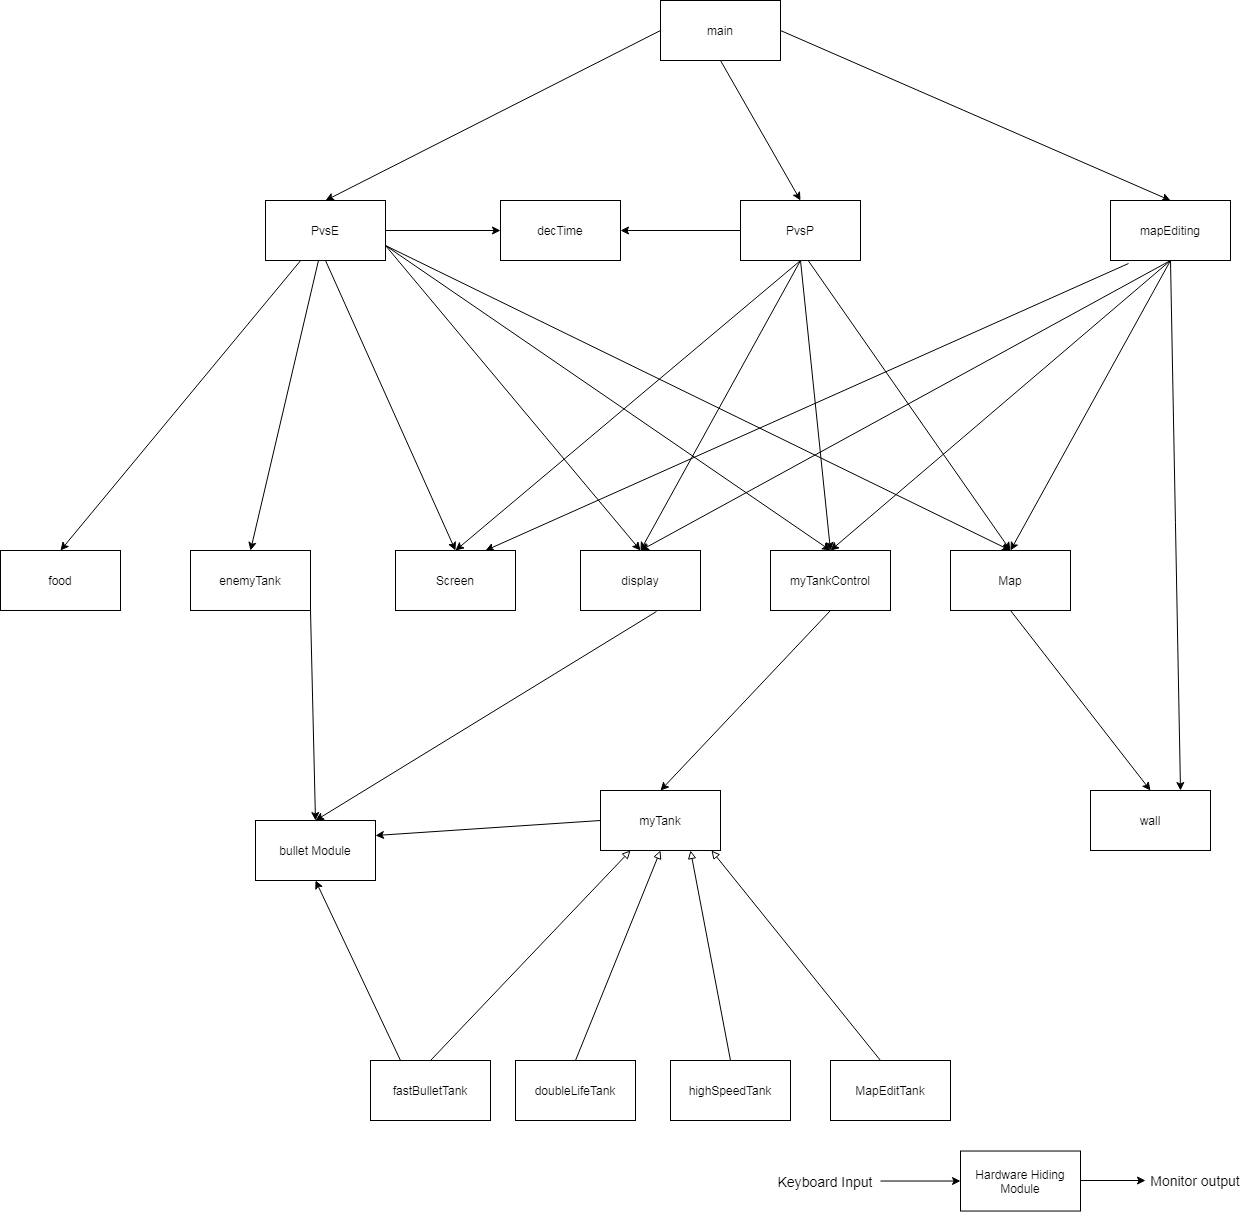
\includegraphics[width=1.05\textwidth]{useHierarchy.png}
\caption{Use hierarchy among modules}
\label{FigUH}
\end{figure}

%\section*{References}

\bibliographystyle {plainnat}
\bibliography {MG}

\end{document}